
\section{Formal Verification of Bitwalker}
\emph{To be done}
\subsection{Verification Objectives}
\emph{To be done}
\subsubsection{Functionality}
\emph{To be done}
\subsubsection{Robustness}
\emph{To be done}

\subsection{The Function \peek}
\label{peek}
\emph{To be done}

\subsubsection{Informal Specification}
\label{informal-peek}


We introduce some auxiliary concepts and formulate general assumptions:

\begin{itemize}
\item
A \emph{bit stream} is an array containing elements of type \verb"uint8_t".

A bit stream of length $n$ contains $8n$ bits.

\item
A bit stream is \emph{valid} if the array is valid.

\item 
A bit stream can be indexed both by its array indices
and its \emph{bit indices}.

Figure~\ref{fig:bitstream-indices} shows the difference between 
array indices and bit indices in a bit stream.
The two bit indices, 0~and~14,
mark bit positions in the first and second array element, respectively.

\begin{figure}[hbt]
\begin{center}
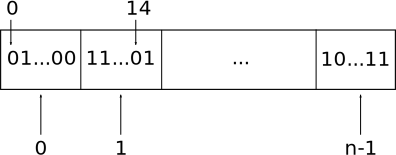
\includegraphics[width=0.40\textwidth]{figures/array_as_stream.pdf}
\caption{\label{fig:bitstream-indices} Array indices and bit indices in a bit stream}
\end{center}
\end{figure}


\item
A \emph{bit sequence} is a consecutive sequence of bits within a bit stream
as represented in Figure~\ref{fig:bitsequence}.
\begin{figure}[hbt]
\begin{center}
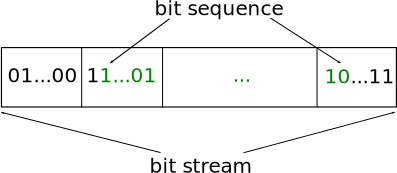
\includegraphics[width=0.40\textwidth]{figures/bit_sequence.pdf}
\caption{\label{fig:bitsequence} A bit sequence within a bit stream}
\end{center}
\end{figure}

A bit sequence is given by the position of its first bit (a bit index in the bit stream)
and its \emph{length}, that is, the number of bits it contains.

\item A bit sequence of length $l$ that starts at bit index $p$ is \emph{valid}
     with respect to a bit stream of length $n$ if the following conditions are
     satisfied
     \begin{align*}
         0 &\leq p \leq 8n \\
         0 &\leq p + l \leq 8n
     \end{align*}

\item 
We assume that the C-types \texttt{unsigned int} and \texttt{int}
have a width of~32~bits.

\end{itemize}

Now we specify \peek with the introduced auxiliary concepts.
The function \texttt{Bitwalker\_Peek} reads a bit sequence from a bit stream
and converts it to an integer.

Its function signature reads as follows:

\begin{lstlisting}[style=acsl-block]
uint64_t  Bitwalker_Peek(unsigned int Startposition, 
                         unsigned int Length,
                         uint8_t Bitstream[],
                         unsigned int BitstreamSizeInBytes);
\end{lstlisting}

The arguments have the following purpose:
\begin{itemize}
    \item \texttt{Startposition} is the bit index in the bit stream 
    where the bit sequence starts.
    \item \texttt{Length} is the length of the bit sequence.
    \item \texttt{Bitstream} is the array which provides the bit stream.
    \item \texttt{BitstreamSizeInBytes} is the length of the array 
    containing the bit stream. 
\end{itemize}


The following preconditions shall hold for the function arguments:
\begin{itemize}
\item \texttt{Bitstream} is a valid array of length \verb"BitstreamSizeInBytes"

\item \texttt{Length} $\leq$ \texttt{64} and

\item \texttt{Startposition + Length} $\leq$ \verb"UINT_MAX".
\end{itemize}

Note that additional constraints are implicitly expressed by the use
of \emph{unsigned} integer types.

We continue with a more precise description of the desired behavior of \peek.
As mentioned, the function \texttt{Bitwalker\_Peek} reads a bit sequence from a bit stream
and converts it to a 64-bit unsigned integer.

The left most bit of the bit sequence is interpreted as
the most significant bit.
Thus, for a bit sequence $(b_0, b_1,\ldots,b_{n - 1})$ the function
returns the sum
\begin{align}
    b_0 \cdot 2^{n - 1} + b_1\cdot 2^{n - 2} + \ldots + b_{n-1}\cdot 2^0
    =
    \sum_{i=0}^{n-1} b_i \cdot 2^{(n - 1) - i} 
\end{align}

If the bit sequence is not valid, then the function returns \texttt{0}.
This increases the robustness of the function.

\subsubsection{Implementation}
\label{impl-peek}
 
Listing~\ref{fig:impl-peek} shows the \isoc implementation of \peek 
for which we aim to verify that it fulfills the informal specification.
The case where the bit sequence is not valid is handled by the \texttt{if}-statement.
For a valid sequence the summation of the bits is done in the \texttt{for}-loop.
The array \texttt{BitwalkerBitMaskTable} is a \texttt{const} helper array 
to select a single bit in the \texttt{Bitstream}.

\begin{listing}[hbt]
\begin{minipage}{\textwidth}
\lstinputlisting[style=acsl-block, frame=single]{./figures/peek.impl}
\end{minipage}
\caption{\label{fig:impl-peek} Implementation of \peek}
\end{listing}

The implementation uses a great amount of bit operations
which is quite a challenge for the formal verification.
We will discuss this further in section~\ref{issues}.

\FloatBarrier

\subsubsection{Formal Specification with \acsl}
\label{formal-peek}

In order to verify that the given implementation of \peek fulfills 
the informal specification, we have to formalize the specification.
Listing~\ref{fig:spec-peek} shows such a formalization in \acsl for \peek.

\begin{listing}[hbt]
\begin{minipage}{\textwidth}
\lstinputlisting[style=acsl-block, frame=single]{./figures/peek.spec}
\end{minipage}
\caption{\label{fig:spec-peek} Formal specification of \peek in \acsl}
\end{listing}

We specify a function contract for \peek containing preconditions
and postconditions introduced by the key words \inl{requires}
and \inl{ensures}, respectively.
In addition, the \acsl language provides the \inl{assigns} clause to specify 
that a function is not allowed to change memory locations other than the ones 
explicitly listed. 
When no \inl{assigns} clauses are specified, 
the function is allowed to modify every visible variable. 

The three preconditions for the function arguments of the informal specification 
are formalized in the function contract by three preconditions.
For the first one we use the predicate \inl{IsValidRange}
which we specified in \acsl in order to state that the \inl{Bitstream}
is a valid array of length \inl{BitstreamSizeInBytes}.
Furthermore, we claim that \peek does not alter any memory locations
apart from internal function variables via the \inl{assigns} clause.

Moreover, we use so-called behaviors in \acsl to describe the two cases
from the informal specification.
The cases are discriminated through the predicate \texttt{ValidBitIndex}.
The first behavior \texttt{out\_of\_range} represents the robustness 
case where the bit sequence is not valid and 
the second behavior specifies the expected behavior in the normal case.

In both cases we state what the result of peek shall be 
as postconditions. In addition, we us a negated form of
a predicate called \inl{TooBig} in the last postcondition of
the normal case. This postcondition was introduced to verify
that the functions \peek and \poke interact correctly.
Therefore, we will discuss this postcondition in section~\ref{interaction}.

Since the implementation of \peek contains a loop,
we also need a loop specification containing a variant for the termination
proof and some invariants to enable the automatic theorem provers
to verify the postconditions.
Although this loop specification is important for the verification,
it is not in the sense to formalize the informal specification.

Since we verify the implementation in accordance to the formal specification, 
it is crucial that it matches the informal one. 
Therefore, we reviewed both specifications.

\FloatBarrier

\subsubsection{Formal Verification with \framac/\wpframac}
\label{verification-peek}


\subsection{The Function \poke}
\label{poke}
\emph{To be done}

\subsubsection{Informal Specification}
\label{informal-poke}



The function \poke converts an integer to a bit sequence and writes it
into a bit stream.
Its function signature reads as follows:
\begin{lstlisting}[style = acsl-block]
int      Bitwalker_Poke(unsigned int Startposition,
                        unsigned int Length,
                        uint8_t Bitstream[],
                        unsigned int BitstreamSizeInBytes,
                        uint64_t Value);
\end{lstlisting}


%\subsubsection*{Arguments}
The arguments have the following purpose:

\begin{itemize}
    \item \texttt{Startposition} is the bit index in the bit stream 
    where the bit sequence starts.
    \item \texttt{Length} is the length of the bit sequence.
    \item \texttt{Bitstream} is the array which provides the bit stream.
    \item \texttt{BitstreamSizeInBytes} is the length of the array 
    containing the bit stream. 
    \item \texttt{Value} is the integer which shall be converted into a bit sequence.
\end{itemize}


%\subsubsection*{Preconditions}
The following preconditions shall hold for the function arguments:

\begin{itemize}
\item \texttt{Bitstream} is a valid array of length \verb"BitstreamSizeInBytes"

\item \texttt{Length} $<$ \texttt{unsigned int}.

\item \texttt{Startposition + Length} $\leq$ \verb"UINT_MAX".
\end{itemize}

Note that additional constraints are implicitly expressed by the use
of \emph{unsigned} integer types.


%\subsubsection*{Description}
Now we can specify \poke as follows:
The function \poke converts a 64-bit unsigned integer to a bit sequence and 
writes it into a bit stream.

For $0 \leq x$ exists a shortest sequence of~0 and~1
$(b_0, b_1,\ldots,b_{n - 1})$
such that
\begin{align}
    \sum_{i=0}^{n-1} b_i \cdot 2^{(n - 1) - i} = x.
\end{align}

The function \poke tries to store the sequence $(b_0, b_1,\ldots,b_{n - 1})$
in the bit sequence of \texttt{Length} bits that starts
at bit index \texttt{Startposition}.

The return value of \poke depends on the following three cases:

\begin{itemize}
\item 
If the bit sequence is valid, then there are two cases:

\begin{itemize}
\item
If $\texttt{Length} \geq n$, then  the sequence
$(\overbrace{0,\ldots,0}^{\texttt{Length}-n},b_0, b_1,\ldots,b_{n - 1})$
is stored in the bit stream starting at \texttt{Startposition}.
The return value of \poke is 0.

\item
If $\texttt{Length} < n$, then the
sequence $(b_0, b_1,\ldots,b_{n - 1})$ cannot be stored and\\
\poke returns~$-2$.
\end{itemize}

\item 
If the bit sequence is not valid, then \poke returns~$-1$.
\end{itemize}

\subsubsection{Implementation}
\label{impl-poke}
Listing \ref{fig:impl-poke} shows the implementation of \poke. The algorithm consists of three cases. The first two matching  the robustness cases
of the informal specification (see subsection Informal Specification~\ref{informal-poke} on page \pageref{informal-poke}) and the last one writhes the bit stream.

\begin{listing}[hbt]
\begin{minipage}{\textwidth}
\lstinputlisting[style=acsl-block, frame=single]{./figures/poke.impl}
\end{minipage}
\caption{\label{fig:impl-poke} Implementation of \poke}
\end{listing}
\FloatBarrier

\subsubsection{Formal Specification with ACSL}

To verify that the implementation meets the informal specification, we need to formalize the it with \acsl. Listing \ref{fig:spec-poke} shows the translated function contract.

The general preconditions of the informal specification are reflected by the  first three  \inl{requires}-clauses at the beginning of the contract.
Because the algorithm modifies the range \inl{Bitstream} and reads the global range  \inl{BitwalkerBitMaskTable} we need to express that the two ranges must use separated memory locations. Therefore we use the predicate \inl{separated} in the fourth \inl{requires}-clause.
Furthermore, in the following \inl{assigns}-clause we must specify the memory locations which altered by the function.


At least, we specify the three behaviors of \poke. The first behavior \inl{out\_of\_range} occurs if the bit sequence between \inl{Starposition} and \inl{Starposition+Length}  not in range \inl{Bitstream}. The postcondition, the return value of the behavior, is formalized with the \inl{requires}-clause.

The second behavior \inl{value\_too\_big} covers the case that \inl{Value} not fits into the given length \inl{Length}.

And finally the behavior \inl{normal} which assumes that the value \inl{Value} is not to big and the bit sequence is in within the range \inl{Bitstream}. Here we assume that the algorithm  only writes to the index positions of \inl{Bitstream} between \inl{Starposition} and \inl{Starposition+Length} and all other memory locations which be used by the array are unaltered.



\begin{listing}[hbt]
\begin{minipage}{\textwidth}
\lstinputlisting[style=acsl-block, frame=single]{./figures/poke.spec}
\end{minipage}
\caption{\label{fig:spec-poke} Formal Specification of \poke}
\end{listing}



\FloatBarrier

\subsubsection{Formal Verification with Frama-C/WP}




\subsection{Interaction of \peek and \poke}
\label{interaction}
\emph{To be done}

\subsubsection{Informal Specification}

The functions \peek and \poke are inverse to each other.


\subsubsection{Implementation}
\subsubsection{Formal Specification with ACSL}
\subsubsection{Formal Verification with Frama-C/WP}



\subsection{Open Issues}
\label{issues}
\emph{To be done}


